\section{Hoe zijn de tussenproducten getest?}
\subsection{Sensoren}
Dit hoofdstuk beschrijft hoe infrarood, ultrasonisch en 9-axis sensoren zijn getest.
\subsubsection{Infrarood sensoren}
\begin{figure}[h]
    \centering
    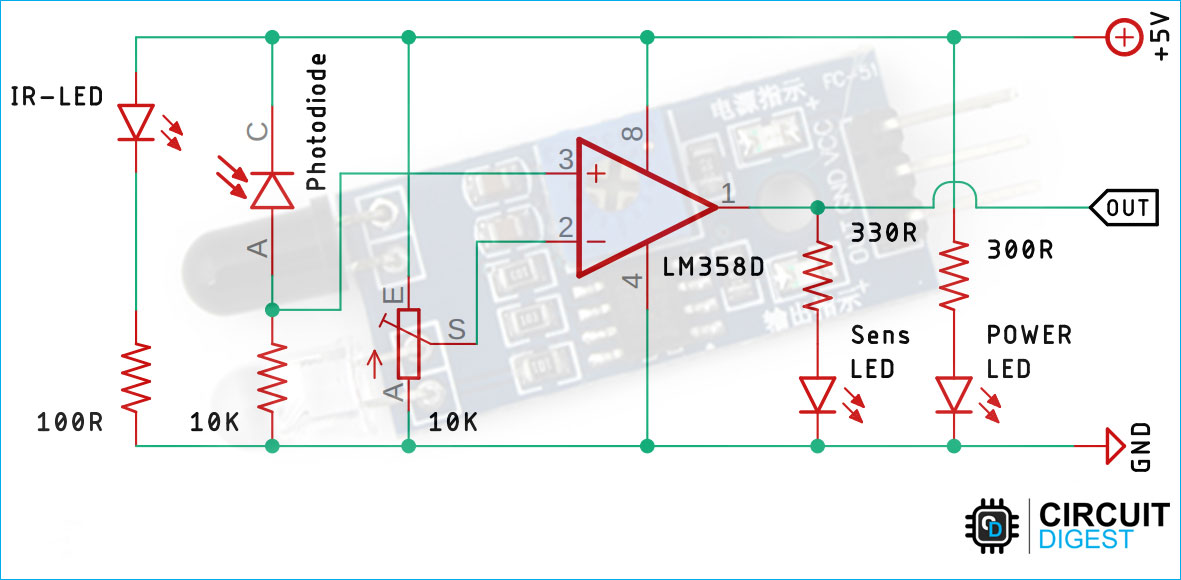
\includegraphics[scale = 0.3]{Media/Figuren/Arduino-IR-Sensor-Circuit.jpg}
    \caption{HW-201 schematische tekening}
    \label{schematic-HW-201}   
    \end{figure}
De infrarood sensor beschikt over drie aansluitingen: VCC, GND en een output pin. De VCC wordt op de 5V aangesloten en de GND pin wordt aangesloten op de grond. Beide pinnen worden aangesloten op de motorshield. De output pin word aangesloten op een willekeurige digitale pin op de Arduino Mega 2560. Voor het inlezen van de infrarood sensor moet op de Arduino mega 2560 de digitale pin worden gedefinieerd als input pin. Later kan met de data iets worden gedaan om objecten te vermijden.

De infrarood sensor beschikt over een LM358 IC\cite{LM358-datasheet} In figuur \eqref{schematic-HW-201}\cite{HW-201-schema} is de schematische tekening te zien van de infrarood sensor. De LM358 vergelijkt twee spanningen op pin 2 en 3, te zien in figuur \eqref{schematic-HW-201}. Afhankelijk van de sterkte van de infrarood straling, komt er een spanning op pin 3 te staan door de fotodiode. Pin 2 is aangesloten op een variabele weerstand. Door aan de variabele weerstand te draaien komt er een andere spanning te staan op pin 2, waarmee de gevoeligheid kan worden ingesteld. Als op pin 3 een hogere spanning komt te staan dan op pin 2, wordt er op pin 1, de output pin, een hoog signaal gegeven. Een laag signaal wordt gegeven als de spanning op pin 3 lager is dan op pin 2.

De infrarood sensor geeft een digitaal signaal op de output pin: 0V of 5V. Voor het meten van de sensoren is gebruik gemaakt van de Seriële monitor in de Arduino IDE met een baudrate van 115200. 

Tijdens het testen werkte twee sensoren niet. Daarvoor zijn er op de oscilloscoop metingen gedaan. Hieruit werd duidelijk dat de sensoren geen 5V genereerden, maar een onbetrouwbare spanning van 2,5V tot 3,5V. Hierna is geconcludeerd dat de sensoren opgeblazen waren, waarna er vervolgens nieuwe infrarood sensoren zijn aangevraagd bij  Ad van den Bergh.

Onder deze alinea bevindt zich de code voor het inlezen van de infrarood sensor. In regel 2 en 3 worden de pinnen van de infrarood sensoren gedefinieerd en wordt het aantal infrarood sensoren opgeslagen om later de data eenvoudig uit te lezen en op te slaan. Vervolgens worden er in regel 5-13 een structure gedefineerd voor de infrarood en ultrasonische sensoren. Voor de infrarood sensor wordt de data voor location[5], state, anglepolarity en sensor\_type[30] respectievelijk locatie, status, hoekpositie en het type sensor gebruikt. Daarna wordt in regel 16-25 een structure aangemaakt met de  meegegeven data. In regel 27-30 is een functie IRstate() aangemaakt voor het uitlezen van de sensorwaardes, waarna de waardes in de structure IR\_sensor worden opgeslagen. Daarna worden in regel 33-35 de infrarood sensoren als input gedefinieerd. Ten slotte kan in regel 38 de functie IRstate() worden aangeroepen.


\begin{lstlisting}
//IR SENSOR
uint8_t IR_pins[] = {2, 3, 4, 5, 6, 7, 8, 9};
uint8_t IR_sensoramount = sizeof(IR_pins) / sizeof(IR_pins[0]);

//Struct data localisation
struct data{
  char location[5];
  int state; //IR
  long duration; //US
  int distance; //US
  int angle; //US
  int anglepolarity; //0 = min, 1 = plus, used for IR
  char sensor_type[30];
};

struct data IR_sensor[] ={
{"RF", 0, 0, 0, 0, 1, "IR Sensor"},
{"LF", 0, 0, 0, 0, 0, "IR Sensor"},
{"LB", 0, 0, 0, 0, 1, "IR Sensor"},
{"RB", 0, 0, 0, 0, 0, "IR Sensor"},
{"RF", 0, 0, 0, 45, 1, "IR Sensor"},
{"LF", 0, 0, 0, 45, 0, "IR Sensor"},
{"LB", 0, 0, 0, 45, 1, "IR Sensor"},
{"RB", 0, 0, 0, 45, 0, "IR Sensor"}
};

void IRstate() { //Reading IR state
  for (int i = 0; i<IR_sensoramount; i++){
    IR_sensor[i].state = digitalRead(IR_pins[i]);
   }}
   
   void setup() {
   for (int i = 0; i<IR_sensoramount; i++){
    pinMode(IR_pins[i], INPUT);
  }}
  
  void loop() {
  IRstate();
  }
\end{lstlisting}
\subsubsection{Ultrasonische sensoren}
De HC-SR04 sensor beschikt over vier pinnen: VCC, GND, trigger en echo. VCC en GND worden op de motorshield voeding aangesloten respectievelijk 5V en grond. De trigger- en echopin wordt aangesloten op een digitale pin van de Arduino mega 2560\cite{HC-SR04}.

De triggerpin is bedoeld om een ultrasonische geluid in de ruimte te sturen door deze pin voor 10 µs hoog te zetten. Nadat de triggerpin laag wordt gezet, wordt de echopin hoog en wacht deze op het ontvangen van het ultrasonisch geluid. Op dit moment wordt de tijd bijgehouden tot het geluid wordt ontvangen. Wanneer er een ultrasonisch geluid wordt ontvangen, wordt de echopin laag. Hieruit kan een afstand worden bepaald, namelijk afstand = snelheid geluid x tijd. Doordat het enige tijd duurt voordat een afstand wordt gemeten, kan een vertraging in de code ontstaan, alhoewel deze miniem zal zijn.

Voor het meten van afstanden van de ultrasonische sensoren is de Seriële monitor  in de Arduino IDE gebruikt met een baudrate van 115200, wat geschikt is voor weergeven van  een afstand tot een object.

Onder deze alinea bevindt zich de code voor het uitlezen en opslaan van de ultrasonische sensor. In regel 2-4 worden de trigger- en echopinnen gedefinieerd, waarbij ook het aantal ultrasoniche sensoren wordt opgeslagen om later eenvoudig de data uit te lezen en op te slaan. Vervolgens wordt in regel 6-14 de structure gedefinieerd voor de infrarood en ultrasonische sensoren. Voor de ultrasonische sensor wordt de data location[5], duration, distance en sensor\_type[30] respectievelijk locatie, duur, afstand en het type sensor gebruikt. Daarna wordt een structure aangemaakt met de meegegeven data. In de regel 22-31 wordt de afstand berekent, waarna het in de structure Sonar\_sensor wordt opgeslagen. Vervolgens worden in regel 33-37 de trigger- en echopin respectievelijk als output en input gedefinieerd. Ten slotte wordt de functie Sonarstate() in regel 39  aangeroepen.
\begin{lstlisting}
//SONAR SENSOR
const int sonartrig_pins[] = {10, 12, 14};
const int sonarecho_pins[] = {11, 13, 15};
int Sonar_sensoramount = sizeof(sonartrig_pins)/sizeof(sonartrig_pins[0]);

//Struct data localisation
struct data{
  char location[5];
  int state; //IR
  long duration; //US
  int distance; //US
  int angle; //US
  int anglepolarity; //0 = min, 1 = plus, used for IR
  char sensor_type[30];
  };
  
  struct data Sonar_sensor[] ={ //declaring 3 sonar sensors 
  {"FRONT", 0, 0, 0, 0, 0, "Sonar sensor"},
  {"LEFT", 0, 0, 0, 0, "Sonar sensor"},
  {"RIGHT", 0, 0, 0, 0, "Sonar sensor"}
  };
  
  void Sonarstate(){ //Reading Sonar state/distance
  for (int i = 0; i<Sonar_sensoramount; i++){
  digitalWrite(sonartrig_pins[i], LOW); 
  delayMicroseconds(2);
  digitalWrite(sonartrig_pins[i], HIGH);  //send a pulse
  delayMicroseconds(10);
  digitalWrite(sonartrig_pins[i], LOW); 
  Sonar_sensor[i].duration = pulseIn(sonarecho_pins[i], HIGH);
  Sonar_sensor[i].distance = Sonar_sensor[i].duration * 0.034 / 2; 
  }}
  
void setup() {
for (int i = 0; i<Sonar_sensoramount; i++){
    pinMode(sonarecho_pins[i], INPUT);
    pinMode(sonartrig_pins[i], OUTPUT);
  }}
  void loop() {
  Sonarstate();  
}

\end{lstlisting}

\subsection{Actuatoren}
\subsubsection{Motoren}
Motorshield
De motoren worden aangestuurd door een motorshield bestaande uit 3 belangrijke coponenten, 2×L293D\cite{h-brug} en 1×74HC595N\cite{shiftregister}. Deze componenten werken samen volgens het volgende diagram.
\begin{figure}[h]
    \centering
    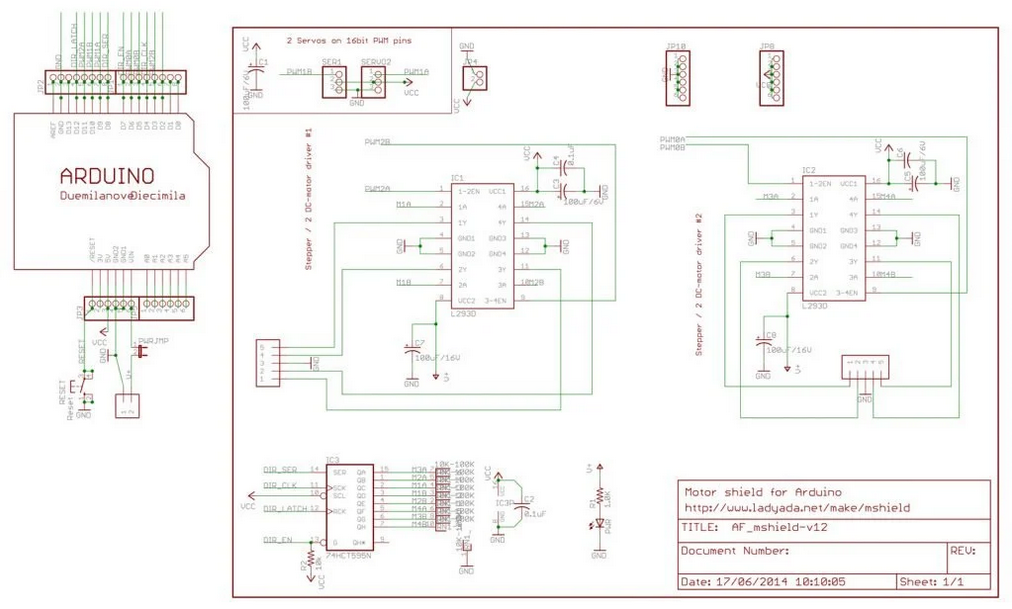
\includegraphics[scale = 0.3]{Media/Figuren/Motorshield_SCHEM.png}
    \caption{Motorshield schematische tekening}
    \label{schematic-Motorshield}   
    \end{figure}

Om het maximale stroomverbruik per kanaal van de H-bruggen te waarborgen, is het totale stroomverbruik per spanning gemeten en zijn vervolgens de resultaten geplot in figuur \ref{Stroomverbruik}. Uit de analyse van de gegevens blijkt dat de motoren niet meer stroom verbruiken dan wat de H-bruggen kunnen verwerken, namelijk 600mA per kanaal. Deze bevindingen zijn van belang omdat ze aangeven dat de H-bruggen veilig en binnen hun capaciteit worden gebruikt in de toepassing van het project.

\begin{figure}[h]
    \centering
    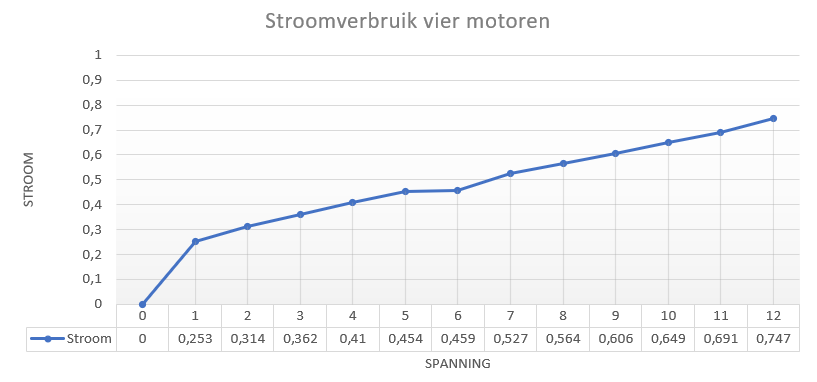
\includegraphics[scale = 0.7]{Media/Figuren/Stroomverbruik.PNG}
    \caption{Stroomverbruik}
    \label{Stroomverbruik}
\end{figure}

\subsubsection{74HC595N Shift Register}
74HC595N\cite{shiftregister} Shift register
De 74HC595N shift register\cite{shiftregister} is een \gls{IC} (Integrated Circuit) dat gebruikt wordt voor het seriele parallelle datatransport. Het IC heeft acht parallelle uitgangen en één seriele ingang. 

Het \gls{IC} heeft 5 ingangen. Het is belangrijk om deze op de juiste momenten aan te sturen, hiervoor heeft Texas Instrument in hun datasheet\cite{shiftregister} een timings \eqref{Timing-register} diagram gemaakt. Hieruit zijn de pinnen makkelijker te ontcijferen en hebben vershillende verschillende pinnen de volgende functies:
\begin{itemize}
    \item Pin 1 (SER): de seriële ingangspen. Hier wordt het seriële signaal dat vanuit de Arduino komt, ingevoerd.
    \item Pin 2 (SRCLK): de shift register klokpen. Hierop wordt een kloksignaal aangesloten dat het verschuiven van de bits in het register triggert.
    \item Pin 3 (RCLK): de latchpen (ook wel register clock genoemd). Hierop wordt een kloksignaal aangesloten dat het overzetten van de inhoud van het shift register naar het output register triggert.
    \item Pin 15 (SRCLR): de shift register clear pen. Hiermee kan het shift register worden gewist.
    \item Pin 16 (OE): de output enable-pen. Hiermee kan de uitgang van het register worden in- of uitgeschakeld.
\end{itemize}
De genoemde ingangen stuur je in de code aan.
\begin{lstlisting}
void MOTOR(int Direction, int MotorPWM1,
int MotorPWM2, int MotorPWM3, int MotorPWM4) {
  SPEED(MotorPWM1, MotorPWM2, MotorPWM3, MotorPWM4);
  digitalWrite(DIR_LATCH, LOW);
  shiftOut(DATA, DIR_CLK, MSBFIRST, Direction);
  digitalWrite(DIR_LATCH, HIGH);}
\end{lstlisting}

\begin{figure} [h]
    \centering
    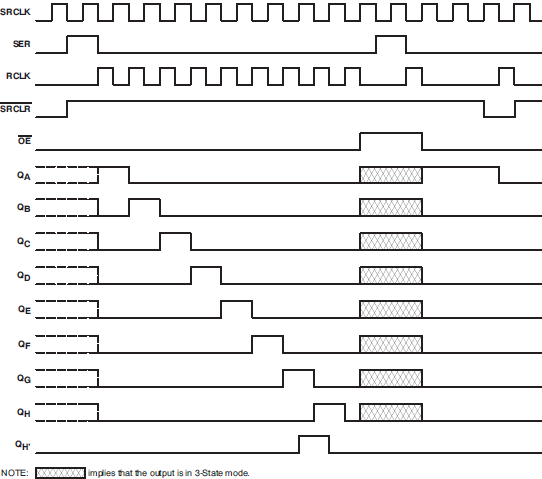
\includegraphics[scale = 0.7]{Media/Figuren/Timing.png}
    \caption{Pin timing \gls{shift-register}}
    \label{Timing-register}   
    \end{figure}
Ook heeft het IC 8 uitgangen, namelijk Q0 t/m Q7, deze zijn verbonden met de L293D. Zie figuur \ref{schematic-Motorshield}.


L293D H-Brug
De L293D\cite{h-brug} is een type H-brug motor driver die de richting en snelheid van DC motoren kan besturen. Het kan tot 600mA aan stroom verwerken en tot twee \gls{DC motoren} tegelijkertijd aansturen. 

De vier ingangspinnen, EN1, EN2, IN1 en IN2, worden gebruikt om de richting en snelheid van de motoren te controleren. 
De uitgangspinnen, OUT1, OUT2, OUT3 en OUT4, zijn verbonden met de motoren. Wanneer de ingangen correct zijn geconfigureerd, kan de L293D\cite{h-brug} de motoren in beide richtingen laten draaien of stoppen. 

De volgende pinnen zijn belangrijk om het IC aan te sturen:
\begin{itemize}
    \item Pin 1, 10 (EN): de enable ingangspinnen. Door een PWM signaal binnen te sturen kan de motorsnelheid aangepast worden.
    \item Pin 11, 6 (IN): de ingangspinnen. Door deze hoog of laag te zetten kan de richting bepaald worden. Deze worden aangestuurd door het \gls{shift-register}\cite{shiftregister}
    \item Pin 2, 5, 9, 12 (OUT): de uitgangspinnen. Deze zijn direct verbonden aan de motoren.
\end{itemize}

\begin{lstlisting}
void SPEED(int MotorPWM1, int MotorPWM2, int MotorPWM3, int MotorPWM4){ 
  analogWrite(PWM2A, MotorPWM1); 
  analogWrite(PWM2B, MotorPWM2);
  analogWrite(PWM0A, MotorPWM3);
  analogWrite(PWM0B, MotorPWM4);}
\end{lstlisting}

Aansturing
Zodra alle datasheets \cite{shiftregister}\cite{h-brug} zijn omgezet in code, kon worden begonnen met het aansturen van de motoren\cite{h-brug}. Gelukkig is de code op een efficiënte manier geschreven, waardoor er functies zijn die op een later moment kunnen worden aangeroepen. 
\begin{lstlisting}
void Forward(){
    MOTOR(DIR_Forward, MotorPWM1, MotorPWM2, MotorPWM3, MotorPWM4);
    displayImage(IMAGES[1]);}
\end{lstlisting}

Om het \gls{motorshield} volledig aan te sturen, is het noodzakelijk om een 8-bits code te verzenden. Deze code is in decimale notatie vastgelegd. Alle beschikbare oriëntatie mogelijkheden zijn opgenomen in tabel 1, figuur \ref{directions}.

\subsubsection{Servo}
Zoals eerder besproken, zijn voor de servo meerdere verschillende versies van de code geschreven. Om te weten of dit werkte moest het getest worden. Het proces van uploaden, uitvoeren, fouten verbeteren en weer herhalen, is het standaard testproces.

Per aanpassing van code werd telkens bepaald wat het verwachtte resultaat was. Vervolgens is de code in een simulator of in de Arduino omgeving geüpload en uitgevoerd. De acties die plaatsvonden zijn vergeleken met het verwachtte resultaat. Werkte dit niet zoals verwacht, dan moest de code worden doorlopen, de fouten worden gelokaliseerd en verbeterd. 

Bij de 1e versie van de servo code ging alles vrij gemakkelijk. Dit was nog een simpele versie, waarbij overigens nog libraries gebruikt waren. Libraries zorgen voor veel simpelere code. Door de functies van de library te gebruiken blijft de code overzichtelijk en zijn de kansen op fouten klein. Bij het testen van deze code is dan ook niet veel fout gegaan. De code werd geüpload naar de Arduino omgeving en uitgevoerd. Hierbij maakte de servo de verwachtte beweging, echter waren de hoeken nog niet naar wens. Dit is toen aangepast waarna het wederom getest werd. 

Voor de 2e versie van de servo code is het standaard proces wederom toegepast. Hierbij moest het proces wel wat vaker herhaald worden om het gewenste resultaat te krijgen, aangezien deze code iets complexer was. 

De 3e versie van de servo code is het meest complex van de drie versies. Hiervoor moest het test proces dan ook vaak herhaald worden. De bedoeling was dat de 3e versie geen delay functies zou bevatten. Om dit voor elkaar te krijgen moest, zoals eerder al uitgelegd, de functie millis() gebruikt worden. Deze functie is aanzienlijk anders dan de eerste twee versies. Na het testproces werkte het echter wel. Toen het in de samengevoegde code werd gezet traden er problemen op. Het resultaat was niet zoals verwacht. De oplossing hiervoor zal nog moeten worden gevonden. 

\subsection{Matrix}
\subsection{Modules}
\subsubsection{Bluetooth}
De HC-05 bluetooth module heeft 6 pinnen, waarvan er vier gebruikt worden voor het besturen van de \gls{Smart-Car}. Dit zijn de pinnen: VCC, GND, \gls{Tx en Rx}. VCC en GND worden aangesloten op de voeding van de Arduino Mega 2560, respectievelijk 5V en GND.  De bluetooth Tx pin wordt aangesloten op de Arduino Mega 2560 Rx1 pin. De bluetooth Rx pin werkt op 3,3V en de Arduino Mega 2560 Tx1 pin op 5V. Hiervoor wordt een spanningsdeling geplaatst met een weerstand van 2000\si{\ohm} en 1000\si{\ohm}. De Arduino Rx1 pin wordt aangesloten op bluetooth Tx pin.

Tijdens het testen bleek dat de bluetooth module een hardwarefout had, waardoor de bluetooth module niet wilde verbinden met een apparaat. Zie figuur \eqref{HC-05 fout}. Als oplossing is er een nieuwe module aangevraagd bij de opdrachtgever
\begin{figure}[h]
    \centering
    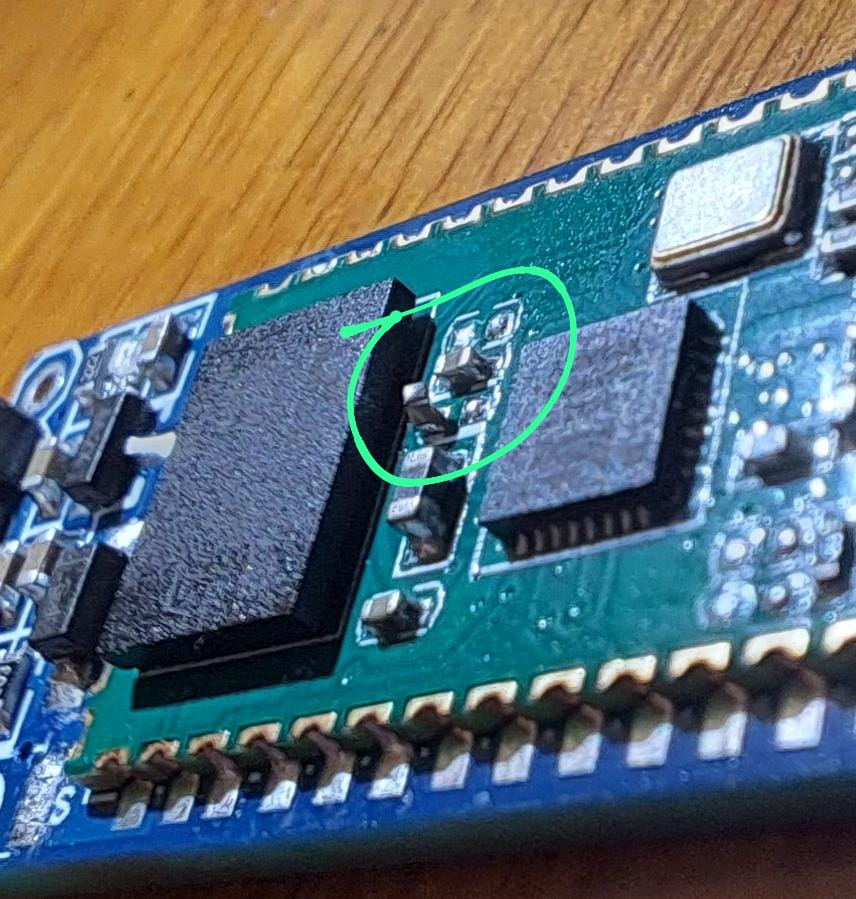
\includegraphics[scale = 0.2]{Media/Figuren/bluetooth hardwarefout.jpg}
    \caption{HC-05 hardwarefout}
    \label{HC-05 fout}
\end{figure}


In de volgende alinea is een eenvoudige code voor het inlezen van bluetooth signalen die vervolgens geprint worden. In het hoofdprogramma worden hier richtingen aan toegekent wat niet wordt weergeven. In regel 5 wordt een variabele aangemaakt die één karakter groot kan zijn. Vervolgens wordt in regel 7-11 de seriële monitor gestart om de richtingen te printen. Daarnaast wordt er een andere seriële monitor gestart waarop de pinnen Tx1 en Rx1 zijn aangesloten, zodat de bluetoothwaarde kan worden uitgelezen. Daarna wordt in regel 15 bekeken of er een waarde is ontvangen door de bluetoothmodule. Als er een waarde is ontvangen, wordt dit in een variabele gezet, te zien in regel 17. Ten slotte wordt in regel 23-43 bij een aantal karakters een taak toegekent.
\newpage
\begin{lstlisting}
char bluetoothValue;

void setup()   {//Here the code only runs once.
  
  Serial.begin(9600);
  Serial1.begin(9600);
}

void loop() {

while(Serial1.available()>0){ 
  
bluetoothValue = Serial1.read();

Serial.print(bluetoothValue);
//Serial.print("\n");
delay(10);

  if(bluetoothValue =='0'){
      Serial.println(" Left ");
  }else if(bluetoothValue == '1'){
      Serial.println(" Forward ");
  }else if(bluetoothValue == '2'){
      Serial.println(" Right ");
  }else if(bluetoothValue == '3'){
      Serial.println(" Backwards ");
  }else if(bluetoothValue == '4'){
      Serial.println(" Faster");
  }else if(bluetoothValue == '5'){
      Serial.println(" Slower");
  }else if(bluetoothValue == '6'){
      Serial.println(" Left rotation");
  }else if(bluetoothValue == '7'){
      Serial.println(" Stop");
  }else if (bluetoothValue == '8'){
      Serial.println(" Right rotation"); 
    }}}
\end{lstlisting}
\subsubsection{RF433MHZ}

\subsection{Zelf rijden}
Onze \gls{Smart-Car} is in staat om zelfstandig te rijden, maar momenteel werkt dit nog niet optimaal. De \gls{Smart-Car} zal continu rechtdoor blijven rijden (zoals beschreven in regel 21), totdat niet meer aan een van de voorwaarden wordt voldaan. Tegelijkertijd controleert de \gls{Smart-Car} of er voldoende ruimte is aan de zijkanten; indien dit niet het geval is, zal hij corrigerend optreden.

In regel 4 en daaropvolgende regels worden de variabelen beschreven die de \gls{Smart-Car} nodig heeft om zichzelf rechtuit te laten rijden met behulp van de BNO055\cite{AXIS}, zoals beschreven in regels 23 tot en met 30.

In het geval dat de ultrasone sensoren een foutieve waarde afgeven en de \gls{Smart-Car} niet in staat is om rechtdoor te rijden maar dit toch blijft doen en dus vast komt te zitten, zal dit worden gedetecteerd en zal de \gls{Smart-Car} zichzelf uit deze situatie bevrijden, zoals beschreven in regels 54 en 55.
\begin{lstlisting}
    int sidecount = 0;
int rotation = 500;
int driven = 0;
float TargetRoll = 0.0;    
float TargetPitch = 0.0;   
float Tolerance = 1.0;
float MovementThreshold = 0.05;   

void selfdrive(){
imu::Vector<3> accel = bno.getVector(Adafruit_BNO055::VECTOR_ACCELEROMETER);

     MotorPWM1 = 90;
     MotorPWM2 = 90;
     MotorPWM3 = 90;
     MotorPWM4 = 90;

  TargetRoll=AXIS_sensor[0].xaxis;
  float RollError = AXIS_sensor[0].xaxis - TargetRoll;
  float PitchError = AXIS_sensor[0].yaxis - TargetPitch;

  if(Sonar_sensor[0].distance>30 || IR_sensor[2].state==0 || IR_sensor[7].state==0)
  {
    if (abs(RollError) <= Tolerance && abs(PitchError) <= Tolerance) {
    // Car is driving straight, use default motor PWM values
    MOTOR(DIR_Forward, MotorPWM1, MotorPWM2, MotorPWM3, MotorPWM4);
    displayImage(IMAGES[1]);
  } else {
    // Car is not driving straight, adjust motor PWM values
    displayImage(IMAGES[1]);
    MOTOR(DIR_Forward, MotorPWM1 - RollError, MotorPWM2 + RollError, MotorPWM3 - RollError, MotorPWM4 + RollError);
  }}else if(sidecount==6){
    Backward(); 
    driven = 1;
    delay(750); 
    sidecount = 0;
      if(Sonar_sensor[1].distance>Sonar_sensor[2].distance){
       Left_Rotation();
       delay(rotation);
      }else if(Sonar_sensor[1].distance<Sonar_sensor[2].distance){
        Right_Rotation();
        delay(rotation);
    }}else if(Sonar_sensor[1].distance>Sonar_sensor[2].distance){
    Left_Sideways();
    sidecount++;
  } else if(Sonar_sensor[1].distance<Sonar_sensor[2].distance){
    Right_Sideways();
    sidecount++;
    } else {STOP();}
if(Sonar_sensor[1].distance<10){
  Right_Sideways();}
if(Sonar_sensor[2].distance<10){
  Left_Sideways();}
    if ((abs(accel.x() - AXIS_sensor[0].LOCXAxis) > MovementThreshold || 
      abs(accel.y() - AXIS_sensor[0].LOCYAxis) > MovementThreshold || AXIS_sensor[0].speed <10) && driven==1 ) {
    Backward(); 
    delay(250);
    driven = 0;
    STOP();
    delay(250);
    Right_Rotation();
    delay(rotation);
      }}
\end{lstlisting}
Om de gemiddelde snelheid van een \gls{Smart-Car} te berekenen, moet de vectoriële som van de acceleratiesnelheden uitgerekend worden.
\begin{equation}
speed = \sqrt{accel.x^2 + accel.y^2 + accel.z^2}
\end{equation}

\subsection{Excelleren}
\subsubsection{Underglow}
Voor het project \gls{Smart-Car} is een underglow verlichting geïnstalleerd en getest. Hierbij zijn een \gls{WS2812B}\cite{WS2812B} ledstrip en een \gls{ESP8266}\cite{ESP8266} gebruikt. Het doel van de verlichting is om de \gls{Smart-Car} te laten opvallen ten opzichte van andere \gls{Smart-Car}'s en om deze een visueel aantrekkelijke uitstraling te geven. Voor het aansturen van de ledstrip is gebruik gemaakt van de \gls{WLED}-bibliotheek.
